\documentclass[11pt]{article}

\usepackage[a4paper,margin=3cm]{geometry} % For page dimensions
\usepackage{fontspec} % For font selection
\usepackage{unicode-math} % For mathematical fonts
\usepackage{polyglossia} % For language selection
\usepackage{graphicx} % For images
\usepackage[colorlinks=true, linkcolor=black, urlcolor=blue, citecolor=green]{hyperref} % For hyperlinks
\usepackage{xcolor} % Colors for code highlighting
\usepackage{fancyhdr} % For headers and footers
\usepackage{bookmark}
\usepackage{nameref} % For referencing sections
\usepackage{draftwatermark} % For watermarks
\usepackage{amsmath} % For mathematical equations
\usepackage{listings} % For code formattings
\usepackage{tikz} % For diagrams

\graphicspath{ {images} }

% Set fonts
% \setmainfont{Noto Serif}
\setromanfont{Noto Serif}
\setsansfont{Noto Sans}
\setmonofont{Noto Sans Mono}

% Set languages
\setmainlanguage{greek}
\setotherlanguages{english}

% Header and footer settings
\pagestyle{fancy}
\setlength{\headheight}{14pt}
\fancyhf{}
\fancyfoot[C]{\thepage}

% Custom Commands
\newcommand{\email}[1]{\href{mailto://#1}{\texttt{#1}}} % Email formatting
\newcommand{\developer}[2]{#1 (#2) \\ \email{up#2@ac.upatras.gr} \\[2ex]}
\newcommand{\appname}{Loop}

\author{
    \developer{Γιάννης Ραβασόπουλος}{1100696}
    \developer{Κώστας Λουκανάρης}{1100610}
    \developer{Χρήστος Μάριος Νικολόπουλος}{1100644}
    \developer{Άγγελος Αβεντισιάν}{1100491}
    \developer{Βασίλης Μυλωνάς}{1100643}
}

\date{
    \today \\[1ex]
    Έκδοση 0.1 \\
}


\fancyhead[L]{Περιπτώσεις Χρήσης}
\fancyhead[R]{\leftmark}

\title{
    Περιπτώσεις Χρήσης - \appname\\[1ex]
    \large Τεχνολογία Λογισμικού - ΤΜΗΥΠ, Πανεπιστήμιο Πατρών \\[2ex]
}

\begin{document}

\maketitle
\thispagestyle{empty}
\newpage

\tableofcontents
\newpage

\begin{abstract}
    Περιγραφή των βασικών οντοτήτων και σχέσεων της εφαρμογής \appname,
\end{abstract}

\newpage


\begin{figure}
    \centering
    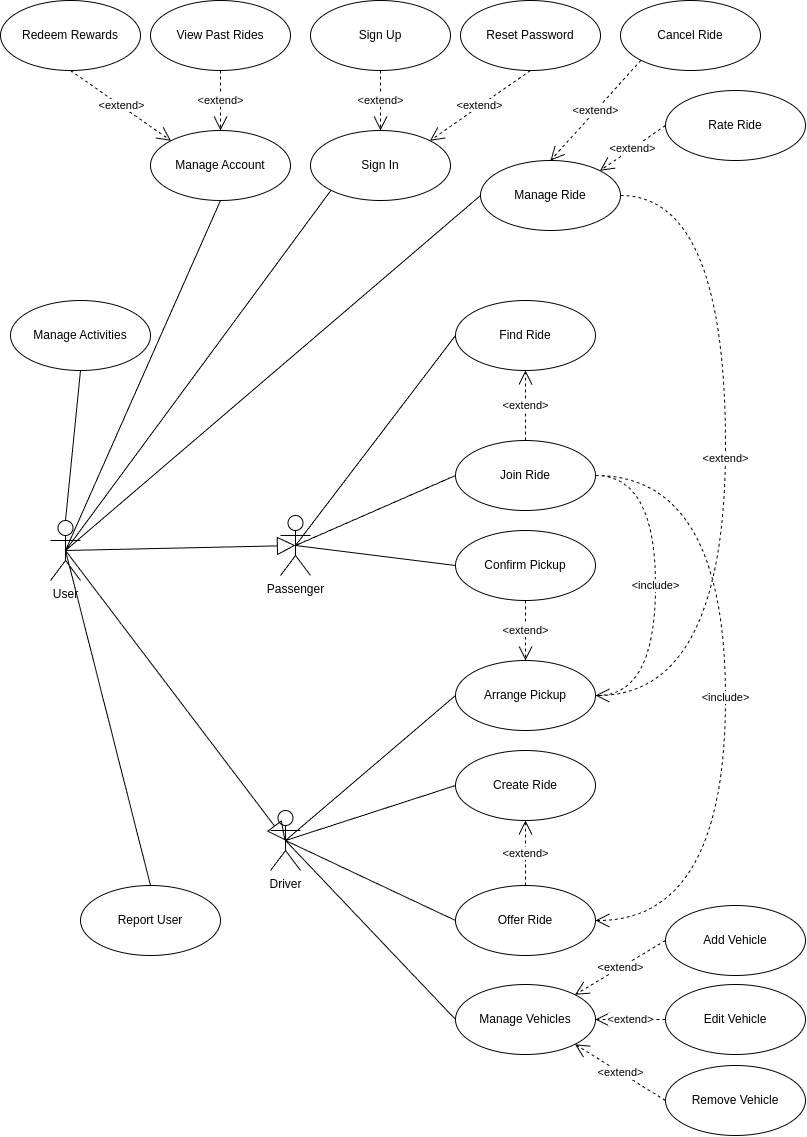
\includegraphics[width=\textwidth]{use-cases.drawio.png}
    \caption{Use Case Diagram}
\end{figure}

\documentclass[11pt]{article}

\usepackage[a4paper,margin=3cm]{geometry} % For page dimensions
\usepackage{fontspec} % For font selection
\usepackage{unicode-math} % For mathematical fonts
\usepackage{polyglossia} % For language selection
\usepackage{graphicx} % For images
\usepackage[colorlinks=true, linkcolor=black, urlcolor=blue, citecolor=green]{hyperref} % For hyperlinks
\usepackage{xcolor} % Colors for code highlighting
\usepackage{fancyhdr} % For headers and footers
\usepackage{bookmark}
\usepackage{nameref} % For referencing sections
\usepackage{draftwatermark} % For watermarks
\usepackage{amsmath} % For mathematical equations
\usepackage{listings} % For code formattings
\usepackage{tikz} % For diagrams

\graphicspath{ {images} }

% Set fonts
% \setmainfont{Noto Serif}
\setromanfont{Noto Serif}
\setsansfont{Noto Sans}
\setmonofont{Noto Sans Mono}

% Set languages
\setmainlanguage{greek}
\setotherlanguages{english}

% Header and footer settings
\pagestyle{fancy}
\setlength{\headheight}{14pt}
\fancyhf{}
\fancyfoot[C]{\thepage}

% Custom Commands
\newcommand{\email}[1]{\href{mailto://#1}{\texttt{#1}}} % Email formatting
\newcommand{\developer}[2]{#1 (#2) \\ \email{up#2@ac.upatras.gr} \\[2ex]}
\newcommand{\appname}{Loop}

\author{
    \developer{Γιάννης Ραβασόπουλος}{1100696}
    \developer{Κώστας Λουκανάρης}{1100610}
    \developer{Χρήστος Μάριος Νικολόπουλος}{1100644}
    \developer{Άγγελος Αβεντισιάν}{1100491}
    \developer{Βασίλης Μυλωνάς}{1100643}
}

\date{
    \today \\[1ex]
    Έκδοση 0.1 \\
}


\fancyhead[L]{Περιπτώσεις Χρήσης}
\fancyhead[R]{\leftmark}

\title{
    Περιπτώσεις Χρήσης - \appname\\[1ex]
    \large Τεχνολογία Λογισμικού - ΤΜΗΥΠ, Πανεπιστήμιο Πατρών \\[2ex]
}

\begin{document}

\maketitle
\thispagestyle{empty}
\newpage

\tableofcontents
\newpage

\begin{abstract}
    Περιγραφή των βασικών οντοτήτων και σχέσεων της εφαρμογής \appname,
\end{abstract}

\newpage

\section{Περιγραφή}

Θεωρούμε ότι σε κάθε βήμα ο χρήστης μπορεί να επιλέξει το πλήκτρο επιστροφής
για να πάει στην προηγούμενη οθόνη.

\subsection{View Past Rides}

Ο χρήστης επιθυμεί να δει το ιστορικό διαδρομών του.

\subsubsection{Βασική ροή}

\begin{enumerate}
    \item Ο χρήστης επιλέγει "Past Rides" στην οθόνη Account.
    \item Το σύστημα ανακτά το ιστορικό διαδρομών και το εμφανίζει στην οθόνη Past Rides.
    \item Ο χρήστης επιλέγει μία διαδρομή στην οθόνη Past Rides.
    \item Το σύστημα εμφανίζει τις λεπτομέρειες της διαδρομής στην οθόνη Ride Details.
\end{enumerate}

\subsubsection{Εναλλακτική Ροή: Διαγραφή διαδρομής από το ιστορικό}

\begin{enumerate}
    \item Ο χρήστης επιλέγει "Delete" στην οθόνη Ride History.
    \item Το σύστημα εμφανίζει τoν διάλογο επιβεβαίωσης διαγραφής.
    \item Ο χρήστης επιλέγει "Confirm" στον διάλογο επιβεβαίωσης διαγραφής.
    \item Το σύστημα διαγράφει τη διαδρομή από το ιστορικό.
    \item Το σύστημα εμφανίζει μήνυμα επιτυχίας στην οθόνη Past Rides.
\end{enumerate}

\subsubsection{Εναλλακτική Ροή: Ακύρωση Διαγραφής}

\begin{enumerate}
    \item Ο χρήστης επιλέγει "Delete" στην οθόνη Ride History.
    \item Το σύστημα εμφανίζει τoν διάλογο επιβεβαίωσης διαγραφής.
    \item Ο χρήστης επιλέγει "Cancel" στον διάλογο επιβεβαίωσης διαγραφής.
    \item Το σύστημα επιστρέφει στην οθόνη Past Rides.
\end{enumerate}

\subsection{Report User}

Ο χρήστης επιθυμεί να αναφέρει έναν άλλο χρήστη της εφαρμογής για παράνομη ή ανεπιθύμητη δραστηριότητα.

\subsubsection{Βασική Ροή}

\begin{enumerate}
    \item Ο χρήστης επιλέγει "Report" στην οθόνη User Details.
    \item Το σύστημα εμφανίζει την φόρμα αναφοράς στην οθόνη Report User.
    \item Ο χρήστης επιλέγει τον λόγο αναφοράς και προσθέτει σχόλια στην οθόνη Report User.
    \item Το σύστημα εμφανίζει τον διάλογο επιβεβαίωσης αναφοράς.
    \item Ο χρήστης επιλέγει "Confirm" στον διάλογο επιβεβαίωσης αναφοράς.
    \item Το σύστημα δημιουργεί την αναφορά.
    \item Το σύστημα καταχωρεί την αναφορά στο αρχείο.
    \item Το σύστημα επεξεργάζεται την αναφορά.
    \item Το σύστημα αναθέτει ποινή στον αναφερόμενο.
    \item Το σύστημα εμφανίζει μήνυμα επιτυχίας στην οθόνη User Details.
\end{enumerate}

\subsubsection{Εναλλακτική Ροή: Απόρριψη Αναφοράς}

\begin{enumerate}
    \item Το σύστημα απορρίπτει την αναφορά.
    \item Το σύστημα εμφανίζει μήνυμα επιτυχίας.
    \item Επιστροφή στην οθόνη User Details.
\end{enumerate}

\subsubsection{Εναλλακτική Ροή: Ακύρωση}

\begin{enumerate}
    \item Ο χρήστης επιλέγει "Cancel" στον διάλογο επιβεβαίωσης αναφοράς.
    \item Το σύστημα επιστρέφει στην οθόνη Report User.
\end{enumerate}


\subsection{Rate User}

Ο χρήστης επιθυμεί να βαθμολογήσει έναν άλλο χρήστη.

\subsubsection{Βασική Ροή}

\begin{enumerate}
    \item Ο χρήστης επιλέγει "Rate" στην οθόνη User Details.
    \item Το σύστημα ελέγχει αν υπάρχει ήδη βαθμολογία στο προφίλ του βαθμολογούμενου.
    \item Η εφαρμογή εμφανίζει την φόρμα βαθμολόγησης στην οθόνη Rate User.
    \item Ο χρήστης επιλέγει την βαθμολογία που θεωρεί και προσθέτει σχόλια στην οθόνη Rate User.
    \item Το σύστημα εμφανίζει τον διάλογο επιβεβαίωσης βαθμολογίας.
    \item Ο χρήστης επιλέγει "Confirm" στον διάλογο επιβεβαίωσης.
    \item Το σύστημα καταχωρεί την βαθμολογία στο προφίλ του βαθμολογούμενου.
    \item Το σύστημα υπολογίζει τη νέα συνολική βαθμολογία του βαθμολογούμενου.
    \item Το σύστημα εμφανίζει μήνυμα επιτυχίας στην οθόνη User Details.
\end{enumerate}

\subsubsection{Εναλλακτική Ροή: Ο χρήστης έχει δώσει βαθμολογία}

\begin{enumerate}
    \item H εφαρμογή εμφανίζει μήνυμα ήδη υπάρχουσας βαθμολογίας στην οθόνη User Details.
\end{enumerate}

\subsubsection{Εναλλακτική Ροή: Ακύρωση}

\begin{enumerate}
    \item Ο χρήστης επιλέγει "Cancel" στον διάλογο επιβεβαίωσης.
    \item Το σύστημα επιστρέφει στην οθόνη User Details.
\end{enumerate}

\subsection{Edit Profile}

Ο χρήστης επιθυμεί να ενημερώσει τα στοιχεία του προφίλ του.

\subsubsection{Βασική Ροή}

\begin{enumerate}
    \item Ο χρήστης επιλέγει "Profile" στην οθόνη Account.
    \item Το σύστημα ανακτά τα στοιχεία προφίλ του χρήστη και τα εμφανίζει στην οθόνη Profile.
    \item Ο χρήστης τροποποιεί κάποια στοιχεία στην οθόνη Profile.
    \item Το σύστημα εμφανίζει τον διάλογο επιβεβαίωσης τροποποίησης.
    \item Ο χρήστης επιλέγει "Confirm" στον διάλογο επιβεβαίωσης τροποποίησης.
    \item Το σύστημα ελέγχει την απάντηση του χρήστη.
    \item Το σύστημα επαληθεύει τα στοιχεία.
    \item To σύστημα ενημερώνει τα στοιχεία προφίλ του χρήστη.
    \item Το σύστημα εμφανίζει μήνυμα επιτυχίας στην οθόνη Account.
\end{enumerate}

\subsubsection{Εναλλακτική Ροή: Ακύρωση}

\begin{enumerate}
    \item Ο χρήστης επιλέγει "Cancel" στον διάλογο επιβεβαίωσης τροποποίησης.
    \item Το σύστημα ελέγχει την απάντηση του χρήστη.
    \item Τo σύστημα επιστρέφει στην οθόνη Account.
\end{enumerate}

\subsubsection{Εναλλακτική Ροή: Αποτυχία Επαλήθευσης}

\begin{enumerate}
    \item Το σύστημα αποτυγχάνει να επαληθεύσει τα στοιχεία.
    \item Το σύστημα εμφανίζει μήνυμα αποτυχίας στην οθόνη Profile.
\end{enumerate}


%

\subsection{Manage Activities}

Ο χρήστης επιθυμεί να διαχειριστεί τις δραστηριότητες του.

\subsubsection{Βασική Ροή}

\begin{enumerate}
    \item[1] Ο χρήστης επιλέγει "Manage Activities".
    \item[2] Η εφαρμογή εμφανίζει τις δραστηριότητες του χρήστη.
\end{enumerate}

\subsubsection{Εναλλακτική Ροή: Δημιουργία δραστηριότητας}

\begin{enumerate}
    \item[3] Ο χρήστης επιλέγει "Create Activity"
    \item[4] Συνέχεια από το βήμα 1 του use case "Create Activity".
\end{enumerate}

\subsubsection{Εναλλακτική Ροή: Τροποποίηση δραστηριότητας}

\begin{enumerate}
    \item[3] Ο χρήστης διαλέγει μια δραστηριότητα και επιλέγει "Edit Activity".
    \item[4] Συνέχεια από το βήμα 1 του use case "Edit Activity".
\end{enumerate}

\subsection{Create Activity}

\subsubsection{Βασική Ροή}

\begin{enumerate}
    \item[1] Ο χρήστης επιλέγει "Create Activity".
    \item[2] Η εφαρμογή εμφανίζει μενού με επιλογές για την ιδιότητα του χρήστη (πχ φοιτητής) την
        περιοχή και τις ώρες μετακίνησης.
    \item[3] Η εφαρμογή εμφανίζει την φόρμα αναζήτησης και έναν χάρτη της περιοχής του χρήστη.
    \item[4] Ο χρήστης επιλέγει την ιδιότητα του.
    \item[5] Ο χρήστης δηλώνει την περιοχή στην οποία επιθυμεί να μετακινηθεί.
    \item[6] Η εφαρμογή εμφανίζει μενού με επιλογές για τις μέρες και τις ώρες έναρξης και λήξης
        της δραστηριότητας.
    \item[7] Ο χρήστης εισάγει τα κατάλληλα στοιχεία.
    \item[8] H εφαρμογή εμφανίζει μενού με επιλογές για το μέσο μεταφοράς του χρήστη
    \item[9] Ο χρήστης επιλέγει το μέσο μεταφοράς του.
    \item[10] Το σύστημα εκτελεί προεπεξεργασία στα δεδομένα.
    \item[11] Το σύστημα εισάγει την δραστηριότητα στο κατάλογο δραστηριοτήτων του χρήστη.
\end{enumerate}

\subsubsection{Εναλλακτική Ροή: Μη έγκυρα στοιχεία}

\begin{enumerate}
    \item[9] Ο χρήστης εισάγει μη έγκυρα στοιχεία.
    \item[10] Το σύστημα εμφανίζει μήνυμα σφάλματος και ζητά διόρθωση.
    \item[11] Ο χρήστης διορθώνει τα στοιχεία.
    \item[12] Συνέχεια από το βήμα 8 της βασικής ροής.
\end{enumerate}

\subsection{Edit Activity}

\subsubsection{Βασική Ροή}

\begin{enumerate}
    \item[1] Η εφαρμογή εμφανίζει τις λεπτομέρειες της δραστηριότητας.
    \item[2] Ο χρήστης τροποποιεί τη δραστηριότητα.
    \item[3] O χρήστης επιλέγει "Save".
    \item[4] Το σύστημα ενημερώνει την δραστηριότητα.
    \item[5] Η εφαρμογή εμφανίζει μήνυμα επιτυχίας.
\end{enumerate}

\subsubsection{Εναλλακτική Ροή: Μη έγκυρα στοιχεία}

\begin{enumerate}
    \item[2] Ο χρήστης εισάγει μη έγκυρα στοιχεία.
    \item[3] Το σύστημα εμφανίζει μήνυμα σφάλματος και ζητά διόρθωση.
    \item[4] Ο χρήστης διορθώνει τα στοιχεία.
    \item[11] Συνέχεια από το βήμα 3 της βασικής ροής.
\end{enumerate}

\subsubsection{Εναλλακτική Ροή: Delete Activity}

\begin{enumerate}
    \item[2] Ο χρήστης επιλέγει "Delete Activity".
    \item[3] Το σύστημα ζητά επιβεβαίωση.
    \item[4] Ο χρήστης επιβεβαιώνει τη διαγραφή.
    \item[5] Το σύστημα διαγράφει την δραστηριότητα από το κατάλογο δραστηριοτήτων του χρήστη.
    \item[6] Το σύστημα εμφανίζει μήνυμα επιτυχίας.
\end{enumerate}

\subsection{Find Ride}

Ένας Carpooler επιθυμεί να βρεί οδηγό με κοινή διαδρομή με αυτόν για να συμμετέχει
σε κάποια δραστηριότητα (εργασία, μάθημα κλπ) ή για να εξυπηρετηθεί εκείνη την
χρονική στιγμή (Insta-Ride).

\subsubsection{Βασική Ροή}

\begin{enumerate}
    \item[1] Ο Carpooler επιλέγει ”Find Ride”.
    \item[2] Η εφαρμογή εμφανίζει τις δραστηριότητες του Carpooler και διάφορες επιλογές.
    \item[3] Ο Carpooler επιλέγει "Insta-Ride".
    \item[4] Η εφαρμογή εμφανίζει μια φόρμα με στοιχεία για το Ride που επιθυμεί.
    \item[5] Ο Carpooler συμπληρώνει τα στοιχεία και πατάει "Confirm".
    \item[6] Το σύστημα αναζητά οδηγούς που εκτελούν διαδρομές που ταιριάζουν.
    \item[7] Το σύστημα κατατάσει τους οδηγούς με βάση το ταίριασμα.
    \item[8] Η εφαρμογή εμφανίζει την λίστα με τους διαθέσιμους οδηγούς.
    \item[9] Ο Carpooler επιλέγει έναν οδηγό.
    \item[10] Η εφαρμογή εμφανίζει περισσότερα στοιχεία για τον οδηγό.
    \item[11] Ο Carpooler επιλέγει "Request Pickup".
    \item[12] Το σύστημα ειδοποιεί τον οδηγό.
    \item[13] Ο οδηγός αποδέχεται την πρόταση.
    \item[14] Συνέχεια από βήμα 1 του use case "Arrange Pickup"
    \item[15] Η εφαρμογή εμφανίζει μήνυμα επιτυχίας και περισσοτερες πληροφορίες για το Pickup. % TODO: confirm?
\end{enumerate}

\subsubsection{Εναλλακτική Ροή: Επιλογή δραστηριότητας}

\begin{enumerate}
    \item[3] O Carpooler επιλέγει μια δραστηριότητα.
    \item[4] Η εφαρμογή εμφανίζει μια προεπισκόπιση της δραστηριότητας.
    \item[5] O Carpooler επιλέγει "Confirm".
    \item[6] Συνέχεια από το βήμα 6 της βασικής ροής.
\end{enumerate}

\subsubsection{Εναλλακτική Ροή: Επιλογή "Manage Activities"}

\begin{enumerate}
    \item[3] O Carpooler επιλέγει "Manage Activities".
    \item[4] Συνέχεια από το βήμα 1 του use case "Manage Activities".
\end{enumerate}

\subsubsection{Εναλλακτική Ροή: Απόρριψη πρότασης από τον οδηγό}

\begin{enumerate}
    \item[13] Ο οδηγός απορρίπτει την πρόταση.
    \item[14] Η εφαρμογή εμφανίζει κατάλληλο μήνυμα στον Carpooler.
    \item[15] Το σύστημα αφαιρεί τον οδηγό από τη λίστα των διαθέσιμων οδηγών.
    \item[16] Συνέχεια από το βήμα 8 της κύριας ροής.
\end{enumerate}

\subsubsection{Εναλλακτική Ροή: Ακύρωση πρότασης από τον Carpooler}

\begin{enumerate}
    \item[12] O Carpooler επιλέγει "Cancel".
    \item[13] Ο επιλεγμένος οδηγός λαμβάνει ειδοποίηση ακύρωσης πρότασης από τον Carpooler.
    \item[14] Συνέχεια από το βήμα 8 της βασικής ροής.
\end{enumerate}

\subsubsection{Εναλλακτική Ροή: Αποτυχία "Arrange Pickup"}

\begin{enumerate}
    \item[14] Η εφαρμογή εμφανίζει μήνυμα αποτυχίας.
    \item[15] Συνέχεια από το βήμα 8 της βασικής ροής.
\end{enumerate}

\subsubsection{Εναλλακτική Ροή: Δεν υπάρχουν διαθέσιμοι οδηγοί}

\begin{enumerate}
    \item[7] Το σύστημα εμφανίζει μήνυμα ότι δεν υπάρχουν διαθέσιμοι οδηγοί.
\end{enumerate}

\newpage

\subsection{Offer Ride}
\label{uc:offer-ride}

Ένας οδηγός κάνει πρόταση για μεταφορά ενός Carpooler.

\subsubsection{Βασική Ροή}

\begin{enumerate}
    \item[1] Ο οδηγός επιλέγει "Offer Ride".
    \item[2] Η εφαρμογή εμφανίζει τις δραστηριότητες του οδηγού και την επιλογή "Insta-Ride".
    \item[3] Ο οδηγός επιλέγει "Insta-Ride".
    \item[4] Η εφαρμογή εμφανίζει μια φόρμα με στοιχεία για το Ride που επιθυμεί.
    \item[5] Ο οδηγός συμπληρώνει τα στοιχεία και πατάει "Confirm".
    \item[6] Η εφαρμογή εμφανίζει μια λίστα με κοντινούς Carpoolers που ταιριάζουν με τη διαδρομή.
    \item[7] Ο οδηγός επιλέγει έναν Carpooler.
    \item[8] Η εφαρμογή εμφανίζει το προφίλ του Carpooler.
    \item[9] Συνέχεια από το βήμα 1 του use case "Arrange Pickup".
    \item[10] Η εφαρμογή εμφανίζει μήνυμα επιτυχίας και περισσότερες πληροφορίες για το Pickup.
\end{enumerate}

\subsubsection{Εναλλακτική Ροή: Επιλογή δραστηριότητας}

\begin{enumerate}
    \item[3] Ο οδηγός επιλέγει μια δραστηριότητα.
    \item[4] Η εφαρμογή εμφανίζει μια προεπισκόπηση της δραστηριότητας.
    \item[5] Ο οδηγός επιλέγει "Confirm".
    \item[6] Η εφαρμογή εμφανίζει μια λίστα με κοντινούς Carpoolers που ταιριάζουν με την
        επιλεγμένη δραστηριότητα.
    \item[7] Συνέχεια από το βήμα 7 της βασικής ροής.
\end{enumerate}

\subsubsection{Εναλλακτική Ροή: Επιλογή "Manage Activities"}

\begin{enumerate}
    \item[3] Ο οδηγός επιλέγει "Manage Activities".
    \item[4] Συνέχεια από το βήμα 1 του use case "Manage Activities".
\end{enumerate}

\subsubsection{Εναλλακτική Ροή: Αποτυχία "Arrange Pickup"}

\begin{enumerate}
    \item[9] Η εφαρμογή εμφανίζει μήνυμα αποτυχίας.
    \item[10] Συνέχεια από το βήμα 6 της βασικής ροής.
\end{enumerate}

\newpage

\subsection{Arrange Pickup}

Ο οδηγός διευθετεί συγκεκριμένα το πότε κι το πού θα γίνει ένα Pickup.

\subsubsection{Βασική Ροή}

\begin{enumerate}
    \item[1] Η εφαρμογή εμφανίζει μια φόρμα για τις πληροφορίες του Pickup.
    \item[2] Ο οδηγός συμπληρώνει την φόρμα.
    \item[3] Ο οδηγός επιλέγει "Submit".
    \item[4] Το σύστημα αποστέλλει την αίτηση Pickup στον Carpooler.
    \item[5] Συνέχεια από βήμα 1 του use case "Accept Pickup"
\end{enumerate}

\subsubsection{Εναλλακτική Ροή: Ελλειπή Στοιχεία}

\begin{enumerate}
    \item[2] Ο οδηγός δεν συμπληρώνει όλα τα υποχρεωτικά πεδία.
    \item[3] Ο οδηγός επιλέγει "Submit".
    \item[4] Η εφαρμογή εμφανίζει μήνυμα σφάλματος και ζητάει συμπλήρωση των στοιχείων.
    \item[5] Ο οδηγός συμπληρώνει τα στοιχεία.
    \item[6] Συνέχεια από το βήμα 3 της βασικής ροής.
\end{enumerate}

\subsubsection{Εναλλακτική Ροή: Ακύρωση}

\begin{enumerate}
    \item[3] Ο οδηγός επιλέγει "Cancel".
\end{enumerate}

\subsection{Accept Pickup}
\label{uc:accept-pickup}

Ένας Carpooler αποδέχεται ή απορρίπτει την αίτηση για Pickup.

\subsubsection{Βασική Ροή}

\begin{enumerate}
    \item[1] Η εφαρμογή εμφανίζει τις πληροφορίες της αίτησης Pickup.
    \item[2] Ο Carpooler επιλέγει "Accept".
    \item[3] Η εφαρμογή εμφανίζει μήνυμα επιτυχίας στον Carpooler.
\end{enumerate}

\subsubsection{Εναλλακτική Ροή: Απόρριψη}

\begin{enumerate}
    \item[2] Ο Carpooler επιλέγει "Reject".
\end{enumerate}

\subsection{Manage Ride}

\subsubsection{Βασική Ροή}

\begin{enumerate}
    \item[1] Ο οδηγός επιλέγει "Manage Ride".
    \item[2] Η εφαρμογή εμφανίζει τα pending και ongoing Rides, τους χρήστες που συμμετέχουν και άλλες
        πληροφορίες.
    \item[3] Ο οδηγός επιλέγει ένα "Ride".
    \item[4] Ο οδηγός επιλέγει "Start Ride".
    \item[5] Η εφαρμογή αλλάζει την κατάσταση του Ride σε "ongoing".
    \item[6] Ο οδηγός επιλέγει έναν Carpooler και πατάει "Pickup".
    \item[7] Το σύστημα επαληθεύει την συνεπιβίβαση.
    \item[8] Ο οδηγός επιλέγει έναν Carpooler και πατάει "Drop Off"
    \item[9] Το σύστημα επαληθεύει την αποβίβαση.
    \item[10] Το σύστημα επιβεβαιώνει την τοποθεσία της αποβίβασης.
    \item[11] Το σύστημα ανανεώνει την βαθμολογία του οδηγού.
    \item[12] Το σύστημα υπολογίζει τους πόντους και τους προσθέτει στο προφίλ του οδηγού.
    \item[13] Ο οδηγός φτάνει στον προορισμό του και επιλέγει "End Ride"
    \item[14] Συνέχεια από το βήμα 1 του use case "Rate User"
    \item[15] To σύστημα ανανεώνει την βαθμολογία των Carpoolers.
\end{enumerate}

\subsubsection{Εναλλακτική Ροή: Ακύρωση από τον οδηγό}

\begin{enumerate}
    \item[4] O οδηγός επιλέγει "Cancel Ride".
    \item[5] Το σύστημα αφαιρεί το "Ride" από την λίστα των pending Rides.
    \item[6] Το σύστημα στέλνει κατάλληλη ειδοποίηση σε τυχόν Carpoolers.
\end{enumerate}

\subsubsection{Εναλλακτική Ροή: Επιβίβαση Carpooler}

\begin{enumerate}
    \item[1] O Carpooler επιλέγει "Manage Ride"
    \item[2] Ο Carpooler επιλέγει "Confirm Pickup".
    \item[3] Το σύστημα επαληθεύει την συνεπιβίβαση.
    \item[4] O Carpooler φτάνει στον προορισμό του και επιλέγει "Confirm Drop Off".
    \item[5] Το σύστημα επαληθεύει την αποβίβαση.
    \item[6] Το σύστημα επιβεβαιώνει την τοποθεσία της αποβίβασης.
    \item[7] Συνέχεια από το βήμα 1 του use case "Rate User"
    \item[8] Το σύστημα ανανεώνει τους πόντους του χρήστη.
\end{enumerate}

\subsubsection{Εναλλακτική Ροή: Ακύρωση από τον Carpooler}

\begin{enumerate}
    \item[1] O Carpooler επιλέγει "Manage Ride"
    \item[2] Η εφαρμογή εμφανίζει τα pending και ongoing Rides, τους χρήστες που συμμετέχουν και άλλες
        πληροφορίες.
    \item[3] Ο οδηγός επιλέγει ένα "Ride".
    \item[4] Ο Carpooler επιλέγει "Cancel Ride".
    \item[5] Το σύστημα αφαιρεί τον Carpooler από το Ride.
    \item[6] Το σύστημα στέλνει κατάλληλη ειδοποίηση στον Οδηγό.
\end{enumerate}

\subsubsection{Εναλλακτική Ροή: Εξαργύρωση πόντων}

\begin{enumerate}
    \item[16] Ο οδηγός επιλέγει "Redeem Reward".
    \item[17] Συνέχεια από το βήμα 1 του use case "Redeem Reward".
\end{enumerate}

\subsubsection{Εναλλακτική Ροή: Αναφορά Χρήστη}

\begin{enumerate}
    \item[16] Ο οδηγός επιλέγει "Report User".
    \item[17] Συνέχεια από το βήμα 1 του use case "Report User".
\end{enumerate}

\newpage

\begin{figure}
    \centering
    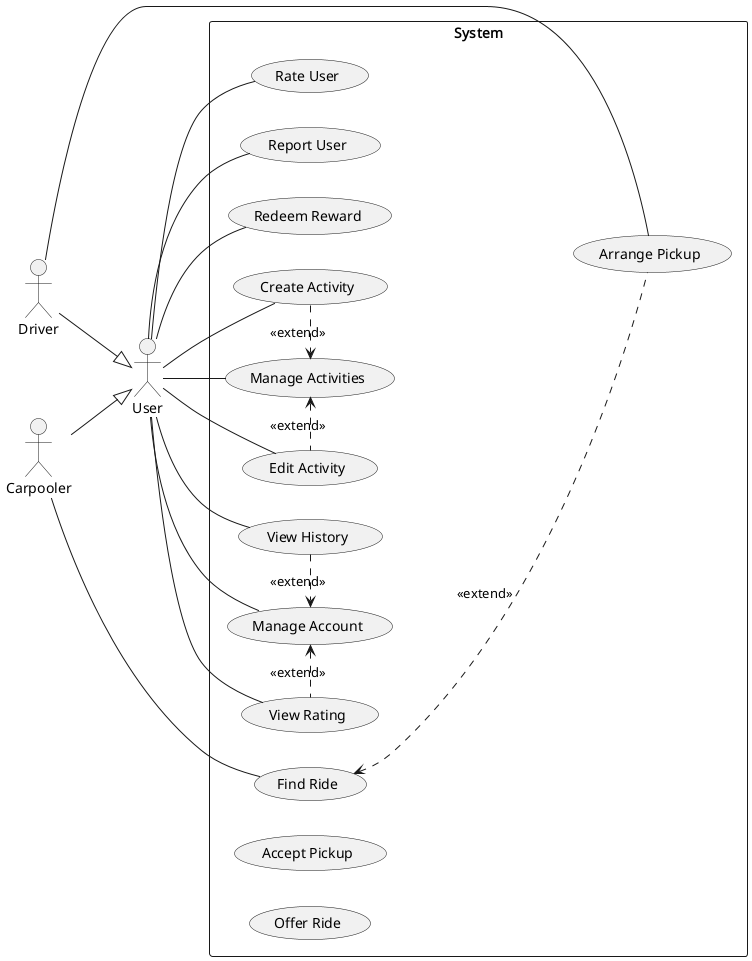
\includegraphics[width=\textwidth]{uml/use-cases}
    \caption{Use Case Diagram}
\end{figure}


\end{document}



% \section{Περιγραφή}

% Θεωρούμε ότι σε κάθε βήμα ο χρήστης μπορεί να επιλέξει το πλήκτρο επιστροφής
% για να πάει στην προηγούμενη οθόνη.

% %

% \subsection{Manage Activities}

% Ο χρήστης επιθυμεί να διαχειριστεί τις δραστηριότητες του.

% \subsubsection{Βασική Ροή}

% \begin{enumerate}
%     \item[1] Ο χρήστης επιλέγει "Manage Activities".
%     \item[2] Η εφαρμογή εμφανίζει τις δραστηριότητες του χρήστη.
% \end{enumerate}

% \subsubsection{Εναλλακτική Ροή: Δημιουργία δραστηριότητας}

% \begin{enumerate}
%     \item[3] Ο χρήστης επιλέγει "Create Activity"
%     \item[4] Συνέχεια από το βήμα 1 του use case "Create Activity".
% \end{enumerate}

% \subsubsection{Εναλλακτική Ροή: Τροποποίηση δραστηριότητας}

% \begin{enumerate}
%     \item[3] Ο χρήστης διαλέγει μια δραστηριότητα και επιλέγει "Edit Activity".
%     \item[4] Συνέχεια από το βήμα 1 του use case "Edit Activity".
% \end{enumerate}

% \subsection{Create Activity}

% \subsubsection{Βασική Ροή}

% \begin{enumerate}
%     \item[1] Ο χρήστης επιλέγει "Create Activity".
%     \item[2] Η εφαρμογή εμφανίζει μενού με επιλογές για την ιδιότητα του χρήστη (πχ φοιτητής) την
%         περιοχή και τις ώρες μετακίνησης.
%     \item[3] Η εφαρμογή εμφανίζει την φόρμα αναζήτησης και έναν χάρτη της περιοχής του χρήστη.
%     \item[4] Ο χρήστης επιλέγει την ιδιότητα του.
%     \item[5] Ο χρήστης δηλώνει την περιοχή στην οποία επιθυμεί να μετακινηθεί.
%     \item[6] Η εφαρμογή εμφανίζει μενού με επιλογές για τις μέρες και τις ώρες έναρξης και λήξης
%         της δραστηριότητας.
%     \item[7] Ο χρήστης εισάγει τα κατάλληλα στοιχεία.
%     \item[8] H εφαρμογή εμφανίζει μενού με επιλογές για το μέσο μεταφοράς του χρήστη
%     \item[9] Ο χρήστης επιλέγει το μέσο μεταφοράς του.
%     \item[10] Το σύστημα εκτελεί προεπεξεργασία στα δεδομένα.
%     \item[11] Το σύστημα εισάγει την δραστηριότητα στο κατάλογο δραστηριοτήτων του χρήστη.
% \end{enumerate}

% \subsubsection{Εναλλακτική Ροή: Μη έγκυρα στοιχεία}

% \begin{enumerate}
%     \item[9] Ο χρήστης εισάγει μη έγκυρα στοιχεία.
%     \item[10] Το σύστημα εμφανίζει μήνυμα σφάλματος και ζητά διόρθωση.
%     \item[11] Ο χρήστης διορθώνει τα στοιχεία.
%     \item[12] Συνέχεια από το βήμα 8 της βασικής ροής.
% \end{enumerate}

% \subsection{Edit Activity}

% \subsubsection{Βασική Ροή}

% \begin{enumerate}
%     \item[1] Η εφαρμογή εμφανίζει τις λεπτομέρειες της δραστηριότητας.
%     \item[2] Ο χρήστης τροποποιεί τη δραστηριότητα.
%     \item[3] O χρήστης επιλέγει "Save".
%     \item[4] Το σύστημα ενημερώνει την δραστηριότητα.
%     \item[5] Η εφαρμογή εμφανίζει μήνυμα επιτυχίας.
% \end{enumerate}

% \subsubsection{Εναλλακτική Ροή: Μη έγκυρα στοιχεία}

% \begin{enumerate}
%     \item[2] Ο χρήστης εισάγει μη έγκυρα στοιχεία.
%     \item[3] Το σύστημα εμφανίζει μήνυμα σφάλματος και ζητά διόρθωση.
%     \item[4] Ο χρήστης διορθώνει τα στοιχεία.
%     \item[11] Συνέχεια από το βήμα 3 της βασικής ροής.
% \end{enumerate}

% \subsubsection{Εναλλακτική Ροή: Delete Activity}

% \begin{enumerate}
%     \item[2] Ο χρήστης επιλέγει "Delete Activity".
%     \item[3] Το σύστημα ζητά επιβεβαίωση.
%     \item[4] Ο χρήστης επιβεβαιώνει τη διαγραφή.
%     \item[5] Το σύστημα διαγράφει την δραστηριότητα από το κατάλογο δραστηριοτήτων του χρήστη.
%     \item[6] Το σύστημα εμφανίζει μήνυμα επιτυχίας.
% \end{enumerate}

% \subsection{Find Ride}

% Ένας Carpooler επιθυμεί να βρεί οδηγό με κοινή διαδρομή με αυτόν για να συμμετέχει
% σε κάποια δραστηριότητα (εργασία, μάθημα κλπ) ή για να εξυπηρετηθεί εκείνη την
% χρονική στιγμή (Insta-Ride).

% \subsubsection{Βασική Ροή}

% \begin{enumerate}
%     \item[1] Ο Carpooler επιλέγει ”Find Ride”.
%     \item[2] Η εφαρμογή εμφανίζει τις δραστηριότητες του Carpooler και διάφορες επιλογές.
%     \item[3] Ο Carpooler επιλέγει "Insta-Ride".
%     \item[4] Η εφαρμογή εμφανίζει μια φόρμα με στοιχεία για το Ride που επιθυμεί.
%     \item[5] Ο Carpooler συμπληρώνει τα στοιχεία και πατάει "Confirm".
%     \item[6] Το σύστημα αναζητά οδηγούς που εκτελούν διαδρομές που ταιριάζουν.
%     \item[7] Το σύστημα κατατάσει τους οδηγούς με βάση το ταίριασμα.
%     \item[8] Η εφαρμογή εμφανίζει την λίστα με τους διαθέσιμους οδηγούς.
%     \item[9] Ο Carpooler επιλέγει έναν οδηγό.
%     \item[10] Η εφαρμογή εμφανίζει περισσότερα στοιχεία για τον οδηγό.
%     \item[11] Ο Carpooler επιλέγει "Request Pickup".
%     \item[12] Το σύστημα ειδοποιεί τον οδηγό.
%     \item[13] Ο οδηγός αποδέχεται την πρόταση.
%     \item[14] Συνέχεια από βήμα 1 του use case "Arrange Pickup"
%     \item[15] Η εφαρμογή εμφανίζει μήνυμα επιτυχίας και περισσοτερες πληροφορίες για το Pickup. % TODO: confirm?
% \end{enumerate}

% \subsubsection{Εναλλακτική Ροή: Επιλογή δραστηριότητας}

% \begin{enumerate}
%     \item[3] O Carpooler επιλέγει μια δραστηριότητα.
%     \item[4] Η εφαρμογή εμφανίζει μια προεπισκόπιση της δραστηριότητας.
%     \item[5] O Carpooler επιλέγει "Confirm".
%     \item[6] Συνέχεια από το βήμα 6 της βασικής ροής.
% \end{enumerate}

% \subsubsection{Εναλλακτική Ροή: Επιλογή "Manage Activities"}

% \begin{enumerate}
%     \item[3] O Carpooler επιλέγει "Manage Activities".
%     \item[4] Συνέχεια από το βήμα 1 του use case "Manage Activities".
% \end{enumerate}

% \subsubsection{Εναλλακτική Ροή: Απόρριψη πρότασης από τον οδηγό}

% \begin{enumerate}
%     \item[13] Ο οδηγός απορρίπτει την πρόταση.
%     \item[14] Η εφαρμογή εμφανίζει κατάλληλο μήνυμα στον Carpooler.
%     \item[15] Το σύστημα αφαιρεί τον οδηγό από τη λίστα των διαθέσιμων οδηγών.
%     \item[16] Συνέχεια από το βήμα 8 της κύριας ροής.
% \end{enumerate}

% \subsubsection{Εναλλακτική Ροή: Ακύρωση πρότασης από τον Carpooler}

% \begin{enumerate}
%     \item[12] O Carpooler επιλέγει "Cancel".
%     \item[13] Ο επιλεγμένος οδηγός λαμβάνει ειδοποίηση ακύρωσης πρότασης από τον Carpooler.
%     \item[14] Συνέχεια από το βήμα 8 της βασικής ροής.
% \end{enumerate}

% \subsubsection{Εναλλακτική Ροή: Αποτυχία "Arrange Pickup"}

% \begin{enumerate}
%     \item[14] Η εφαρμογή εμφανίζει μήνυμα αποτυχίας.
%     \item[15] Συνέχεια από το βήμα 8 της βασικής ροής.
% \end{enumerate}

% \subsubsection{Εναλλακτική Ροή: Δεν υπάρχουν διαθέσιμοι οδηγοί}

% \begin{enumerate}
%     \item[7] Το σύστημα εμφανίζει μήνυμα ότι δεν υπάρχουν διαθέσιμοι οδηγοί.
% \end{enumerate}

% \newpage

% \subsection{Offer Ride}
% \label{uc:offer-ride}

% Ένας οδηγός κάνει πρόταση για μεταφορά ενός Carpooler.

% \subsubsection{Βασική Ροή}

% \begin{enumerate}
%     \item[1] Ο οδηγός επιλέγει "Offer Ride".
%     \item[2] Η εφαρμογή εμφανίζει τις δραστηριότητες του οδηγού και την επιλογή "Insta-Ride".
%     \item[3] Ο οδηγός επιλέγει "Insta-Ride".
%     \item[4] Η εφαρμογή εμφανίζει μια φόρμα με στοιχεία για το Ride που επιθυμεί.
%     \item[5] Ο οδηγός συμπληρώνει τα στοιχεία και πατάει "Confirm".
%     \item[6] Η εφαρμογή εμφανίζει μια λίστα με κοντινούς Carpoolers που ταιριάζουν με τη διαδρομή.
%     \item[7] Ο οδηγός επιλέγει έναν Carpooler.
%     \item[8] Η εφαρμογή εμφανίζει το προφίλ του Carpooler.
%     \item[9] Συνέχεια από το βήμα 1 του use case "Arrange Pickup".
%     \item[10] Η εφαρμογή εμφανίζει μήνυμα επιτυχίας και περισσότερες πληροφορίες για το Pickup.
% \end{enumerate}

% \subsubsection{Εναλλακτική Ροή: Επιλογή δραστηριότητας}

% \begin{enumerate}
%     \item[3] Ο οδηγός επιλέγει μια δραστηριότητα.
%     \item[4] Η εφαρμογή εμφανίζει μια προεπισκόπηση της δραστηριότητας.
%     \item[5] Ο οδηγός επιλέγει "Confirm".
%     \item[6] Η εφαρμογή εμφανίζει μια λίστα με κοντινούς Carpoolers που ταιριάζουν με την
%         επιλεγμένη δραστηριότητα.
%     \item[7] Συνέχεια από το βήμα 7 της βασικής ροής.
% \end{enumerate}

% \subsubsection{Εναλλακτική Ροή: Επιλογή "Manage Activities"}

% \begin{enumerate}
%     \item[3] Ο οδηγός επιλέγει "Manage Activities".
%     \item[4] Συνέχεια από το βήμα 1 του use case "Manage Activities".
% \end{enumerate}

% \subsubsection{Εναλλακτική Ροή: Αποτυχία "Arrange Pickup"}

% \begin{enumerate}
%     \item[9] Η εφαρμογή εμφανίζει μήνυμα αποτυχίας.
%     \item[10] Συνέχεια από το βήμα 6 της βασικής ροής.
% \end{enumerate}

% \newpage


% \subsection{Accept Pickup}
% \label{uc:accept-pickup}

% Ένας Carpooler αποδέχεται ή απορρίπτει την αίτηση για Pickup.

% \subsubsection{Βασική Ροή}

% \begin{enumerate}
%     \item[1] Η εφαρμογή εμφανίζει τις πληροφορίες της αίτησης Pickup.
%     \item[2] Ο Carpooler επιλέγει "Accept".
%     \item[3] Η εφαρμογή εμφανίζει μήνυμα επιτυχίας στον Carpooler.
% \end{enumerate}

% \subsubsection{Εναλλακτική Ροή: Απόρριψη}

% \begin{enumerate}
%     \item[2] Ο Carpooler επιλέγει "Reject".
% \end{enumerate}

% \subsection{Manage Ride}

% \subsubsection{Βασική Ροή}

% \begin{enumerate}
%     \item[1] Ο οδηγός επιλέγει "Manage Ride".
%     \item[2] Η εφαρμογή εμφανίζει τα pending και ongoing Rides, τους χρήστες που συμμετέχουν και άλλες
%         πληροφορίες.
%     \item[3] Ο οδηγός επιλέγει ένα "Ride".
%     \item[4] Ο οδηγός επιλέγει "Start Ride".
%     \item[5] Η εφαρμογή αλλάζει την κατάσταση του Ride σε "ongoing".
%     \item[6] Ο οδηγός επιλέγει έναν Carpooler και πατάει "Pickup".
%     \item[7] Το σύστημα επαληθεύει την συνεπιβίβαση.
%     \item[8] Ο οδηγός επιλέγει έναν Carpooler και πατάει "Drop Off"
%     \item[9] Το σύστημα επαληθεύει την αποβίβαση.
%     \item[10] Το σύστημα επιβεβαιώνει την τοποθεσία της αποβίβασης.
%     \item[11] Το σύστημα ανανεώνει την βαθμολογία του οδηγού.
%     \item[12] Το σύστημα υπολογίζει τους πόντους και τους προσθέτει στο προφίλ του οδηγού.
%     \item[13] Ο οδηγός φτάνει στον προορισμό του και επιλέγει "End Ride"
%     \item[14] Συνέχεια από το βήμα 1 του use case "Rate User"
%     \item[15] To σύστημα ανανεώνει την βαθμολογία των Carpoolers.
% \end{enumerate}

% \subsubsection{Εναλλακτική Ροή: Ακύρωση από τον οδηγό}

% \begin{enumerate}
%     \item[4] O οδηγός επιλέγει "Cancel Ride".
%     \item[5] Το σύστημα αφαιρεί το "Ride" από την λίστα των pending Rides.
%     \item[6] Το σύστημα στέλνει κατάλληλη ειδοποίηση σε τυχόν Carpoolers.
% \end{enumerate}

% \subsubsection{Εναλλακτική Ροή: Επιβίβαση Carpooler}

% \begin{enumerate}
%     \item[1] O Carpooler επιλέγει "Manage Ride"
%     \item[2] Ο Carpooler επιλέγει "Confirm Pickup".
%     \item[3] Το σύστημα επαληθεύει την συνεπιβίβαση.
%     \item[4] O Carpooler φτάνει στον προορισμό του και επιλέγει "Confirm Drop Off".
%     \item[5] Το σύστημα επαληθεύει την αποβίβαση.
%     \item[6] Το σύστημα επιβεβαιώνει την τοποθεσία της αποβίβασης.
%     \item[7] Συνέχεια από το βήμα 1 του use case "Rate User"
%     \item[8] Το σύστημα ανανεώνει τους πόντους του χρήστη.
% \end{enumerate}

% \subsubsection{Εναλλακτική Ροή: Ακύρωση από τον Carpooler}

% \begin{enumerate}
%     \item[1] O Carpooler επιλέγει "Manage Ride"
%     \item[2] Η εφαρμογή εμφανίζει τα pending και ongoing Rides, τους χρήστες που συμμετέχουν και άλλες
%         πληροφορίες.
%     \item[3] Ο οδηγός επιλέγει ένα "Ride".
%     \item[4] Ο Carpooler επιλέγει "Cancel Ride".
%     \item[5] Το σύστημα αφαιρεί τον Carpooler από το Ride.
%     \item[6] Το σύστημα στέλνει κατάλληλη ειδοποίηση στον Οδηγό.
% \end{enumerate}

% \subsubsection{Εναλλακτική Ροή: Εξαργύρωση πόντων}

% \begin{enumerate}
%     \item[16] Ο οδηγός επιλέγει "Redeem Reward".
%     \item[17] Συνέχεια από το βήμα 1 του use case "Redeem Reward".
% \end{enumerate}

% \subsubsection{Εναλλακτική Ροή: Αναφορά Χρήστη}

% \begin{enumerate}
%     \item[16] Ο οδηγός επιλέγει "Report User".
%     \item[17] Συνέχεια από το βήμα 1 του use case "Report User".
% \end{enumerate}

% \newpage

\end{document}
